\documentclass[11pt,a4paper]{article}

\usepackage[spanish,es-noquoting]{babel}
\usepackage[utf8]{inputenc}
\usepackage[T1]{fontenc}
\usepackage{lmodern}
\usepackage{geometry}
\usepackage{booktabs}
\usepackage{tabularx}
\usepackage{longtable}
\usepackage{array}
\usepackage{multirow}
\usepackage{float}
\usepackage{graphicx}
\usepackage{enumitem}
\usepackage{hyperref}
\usepackage{xcolor}
\usepackage{colortbl}
\usepackage{fancyhdr}
\usepackage{caption}
\usepackage{subcaption}
\usepackage{amsmath}

\geometry{margin=2.5cm}
\setlength{\parskip}{0.5em}
\setlength{\parindent}{0pt}
\hypersetup{colorlinks=true, linkcolor=black, urlcolor=blue}

\definecolor{malignored}{RGB}{231,76,60}
\definecolor{benigngreen}{RGB}{46,204,113}
\definecolor{lightgray}{RGB}{245,245,245}
\definecolor{medgray}{RGB}{220,220,220}
\definecolor{darkblue}{RGB}{41,128,185}

\setlength{\headheight}{14pt}
\pagestyle{fancy}
\fancyhf{}
\lhead{\textit{Proyecto 2 -- Data Mining}}
\rhead{\textit{Semana 1: EDA}}
\cfoot{\thepage}
\renewcommand{\headrulewidth}{0.4pt}

\title{\textbf{Proyecto 2 -- Data Mining}\\[0.4em]
       \large Semana 1: Comprensión del Problema y Análisis Exploratorio de Datos}
\author{Javier España \and Ángel Esquit \and Roberto Barreda \and Diego López}
\date{Abril 2026}

\begin{document}

\maketitle
\thispagestyle{empty}

\begin{center}
\large Universidad del Valle de Guatemala\\[0.2em]
\normalsize Curso: Data Mining \quad|\quad Dataset: Wisconsin Breast Cancer Dataset\\[0.2em]
Variable objetivo: \texttt{Class} \;(2 = Benigno, 4 = Maligno)
\end{center}

\vspace{0.5em}\hrule\vspace{0.5em}

\tableofcontents
\newpage

% ─────────────────────────────────────────────
\section{Contexto del Problema}
% ─────────────────────────────────────────────

El cáncer de mama es la neoplasia maligna más frecuente en mujeres a nivel mundial. La detección temprana mediante biopsia por aspiración con aguja fina (FNA) es un procedimiento mínimamente invasivo que extrae células de una masa mamaria para evaluación citológica. El dataset de trabajo captura el resultado de ese proceso: cada registro representa una muestra analizada por un patólogo, con 9 características de morfología celular puntuadas en escala 1--10.

\textbf{Problema a resolver:} clasificación binaria supervisada para predecir si un tumor es \textbf{benigno} (Clase 2) o \textbf{maligno} (Clase 4) a partir de esas características. El fallo más costoso es el \textit{falso negativo}: clasificar un tumor maligno como benigno puede retrasar el tratamiento con consecuencias graves. Esto condiciona todas las decisiones metodológicas del proyecto: la métrica principal de evaluación será el \textbf{Recall de la clase maligna}, no la exactitud global.

% ─────────────────────────────────────────────
\section{Descripción del Conjunto de Datos}
% ─────────────────────────────────────────────

El archivo \texttt{Datos.csv} proviene del \textit{Wisconsin Breast Cancer Dataset} (Dr.\ William H.\ Wolberg, Universidad de Wisconsin), uno de los datasets de referencia en clasificación médica con aprendizaje automático.

\subsection{Dimensiones y estructura}

\begin{table}[H]
\centering
\caption{Resumen estructural del dataset original}
\begin{tabular}{lc}
\toprule
\textbf{Característica} & \textbf{Valor} \\
\midrule
Total de registros & 683 \\
Variables predictoras & 9 \\
Variable objetivo & 1 (\texttt{Class}) \\
Identificador (no predictivo) & 1 (\texttt{Sample code number}) \\
Total de columnas & 11 \\
Valores nulos & 0 \\
Registros duplicados & 8 \\
Rango de variables predictoras & 1 -- 10 (ordinal) \\
\bottomrule
\end{tabular}
\end{table}

\subsection{Diccionario de variables}

\begin{table}[H]
\centering
\caption{Variables del dataset, tipo, rango e interpretación clínica}
\renewcommand{\arraystretch}{1.2}
\begin{tabularx}{\textwidth}{l l c X}
\toprule
\textbf{Variable} & \textbf{Tipo} & \textbf{Rango} & \textbf{Descripción / Significado clínico} \\
\midrule
\rowcolor{lightgray}
Sample code number & ID entero & --- & Identificador único de muestra; excluido del modelado \\
Clump Thickness & Ordinal & 1--10 & Grosor del grupo celular; mayor valor indica aglomeración anormal \\
\rowcolor{lightgray}
Uniformity of Cell Size & Ordinal & 1--10 & Uniformidad de tamaño entre células; alta variabilidad es señal de malignidad \\
Uniformity of Cell Shape & Ordinal & 1--10 & Uniformidad de forma celular; morfología irregular asociada a malignidad \\
\rowcolor{lightgray}
Marginal Adhesion & Ordinal & 1--10 & Adhesión al tejido circundante; células malignas tienden a desprenderse \\
Single Epithelial Cell Size & Ordinal & 1--10 & Tamaño de célula epitelial individual; agrandamiento celular es señal atípica \\
\rowcolor{lightgray}
Bare Nuclei & Ordinal & 1--10 & Núcleos sin citoplasma visible; marcador fuerte de malignidad \\
Bland Chromatin & Ordinal & 1--10 & Textura de la cromatina nuclear; cromatina gruesa es indicador de malignidad \\
\rowcolor{lightgray}
Normal Nucleoli & Ordinal & 1--10 & Tamaño y número de nucléolos; nucléolos prominentes indican actividad mitótica \\
Mitoses & Ordinal & 1--10 & Frecuencia de divisiones celulares; alta mitosis es criterio diagnóstico de malignidad \\
\rowcolor{lightgray}
Class & Binaria & \{2, 4\} & \textbf{Variable objetivo}: 2 = Benigno, 4 = Maligno \\
\bottomrule
\end{tabularx}
\end{table}

% ─────────────────────────────────────────────
\section{Análisis Exploratorio de Datos (EDA)}
% ─────────────────────────────────────────────

\subsection{Distribución de la variable objetivo}

Se observó un \textbf{desbalance moderado} de clases: 65.0\% benignos frente a 35.0\% malignos.

\begin{table}[H]
\centering
\caption{Distribución de la variable objetivo}
\begin{tabular}{lcc}
\toprule
\textbf{Clase} & \textbf{Frecuencia} & \textbf{Porcentaje} \\
\midrule
\rowcolor{benigngreen!20}
2 -- Benigno & 444 & 65.0\% \\
\rowcolor{malignored!20}
4 -- Maligno & 239 & 35.0\% \\
\midrule
Total & 683 & 100.0\% \\
\bottomrule
\end{tabular}
\end{table}

Un clasificador ingenuo que predijera siempre ``Benigno'' obtendría un 65\% de exactitud, lo que demuestra que la \textit{accuracy} sola es una métrica engañosa para este problema. \textbf{Decisión metodológica:} se usará \texttt{class\_weight=`balanced'} en los modelos lineales para compensar el desbalance. No se aplicará SMOTE porque el ratio 1.86:1 no es severo y se prioriza no introducir muestras sintéticas en un dataset pequeño con datos clínicos reales.

\begin{figure}[H]
\centering
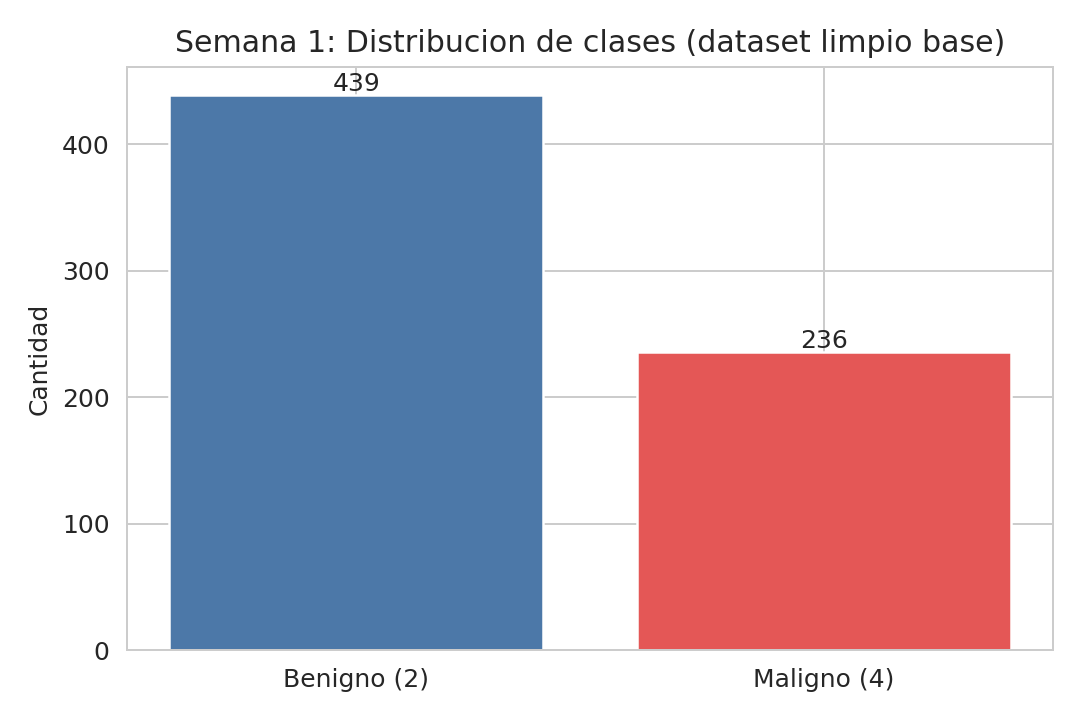
\includegraphics[width=0.62\textwidth]{figures/s1_distribucion_clases.png}
\caption{Distribución de clases en el dataset. El desbalance moderado (1.86:1) condiciona la selección de métricas de evaluación.}
\end{figure}

\subsection{Estadísticas descriptivas por variable}

\begin{table}[H]
\centering
\caption{Estadísticas descriptivas de las variables predictoras (683 registros)}
\small
\renewcommand{\arraystretch}{1.1}
\begin{tabular}{lcccccccc}
\toprule
\textbf{Variable} & \textbf{Media} & \textbf{Desv.\ Est.} & \textbf{Min} & \textbf{Q1} & \textbf{Mediana} & \textbf{Q3} & \textbf{Max} \\
\midrule
Clump Thickness & 4.44 & 2.82 & 1 & 2 & 4 & 6 & 10 \\
Uniformity of Cell Size & 3.15 & 3.07 & 1 & 1 & 1 & 5 & 10 \\
Uniformity of Cell Shape & 3.22 & 2.99 & 1 & 1 & 1 & 5 & 10 \\
Marginal Adhesion & 2.83 & 2.86 & 1 & 1 & 1 & 4 & 10 \\
Single Epithelial Cell Size & 3.23 & 2.22 & 1 & 2 & 2 & 4 & 10 \\
Bare Nuclei & 3.54 & 3.64 & 1 & 1 & 1 & 6 & 10 \\
Bland Chromatin & 3.45 & 2.45 & 1 & 2 & 3 & 5 & 10 \\
Normal Nucleoli & 2.87 & 3.05 & 1 & 1 & 1 & 4 & 10 \\
Mitoses & 1.60 & 1.73 & 1 & 1 & 1 & 1 & 10 \\
\bottomrule
\end{tabular}
\normalsize
\end{table}

Las medianas bajas (Q2 = 1 en la mayoría de variables) reflejan que la mayor parte de la distribución corresponde a casos benignos. La alta desviación estándar en variables como \texttt{Bare Nuclei} (3.64) y \texttt{Uniformity of Cell Size} (3.07) anticipa que existirá separación significativa entre clases.

\subsection{Diferencia de medias por diagnóstico}

\begin{table}[H]
\centering
\caption{Media por variable según clase diagnóstica y diferencia absoluta}
\renewcommand{\arraystretch}{1.15}
\begin{tabular}{lcccc}
\toprule
\textbf{Variable} & \textbf{Benigno (media)} & \textbf{Maligno (media)} & \textbf{$\Delta$ (Mal $-$ Ben)} \\
\midrule
\rowcolor{malignored!15}
Bare Nuclei & 1.35 & 7.63 & \textbf{+6.28} \\
\rowcolor{malignored!15}
Uniformity of Cell Size & 1.31 & 6.58 & \textbf{+5.27} \\
\rowcolor{malignored!15}
Uniformity of Cell Shape & 1.41 & 6.56 & \textbf{+5.15} \\
Clump Thickness & 2.96 & 7.19 & +4.23 \\
Marginal Adhesion & 1.35 & 5.59 & +4.24 \\
Normal Nucleoli & 1.26 & 5.86 & +4.60 \\
Bland Chromatin & 2.08 & 5.97 & +3.89 \\
Single Epithelial Cell Size & 2.11 & 5.33 & +3.22 \\
Mitoses & 1.07 & 2.60 & +1.53 \\
\bottomrule
\end{tabular}
\end{table}

Las tres variables con mayor diferencia de medias (\texttt{Bare Nuclei}, \texttt{Uniformity of Cell Size} y \texttt{Uniformity of Cell Shape}) son precisamente las más correlacionadas con la clase objetivo. \texttt{Mitoses} muestra la menor diferencia y es, consistentemente, la variable menos discriminativa del dataset.

\subsection{Distribución de características por clase}

Los histogramas por diagnóstico confirman el patrón observado en las medias: \textbf{los casos benignos se concentran fuertemente en valores bajos (1--3)}, mientras que los malignos presentan distribuciones más dispersas y sesgadas hacia valores altos.

\begin{figure}[H]
\centering
\includegraphics[width=\textwidth]{figures/s1_histogramas_por_clase.png}
\caption{Distribución de cada variable predictora segmentada por diagnóstico (verde = Benigno, rojo = Maligno). Las tres primeras variables del panel superior muestran la separación más marcada.}
\end{figure}

Un fenómeno relevante es el \textbf{efecto techo}: varias variables malignas acumulan observaciones en el valor máximo (10). Esto indica que la escala puede ser insuficiente para representar casos extremos y que algunos outliers son casos clínicamente severos, no errores de medición.

\subsection{Correlaciones entre variables y con la clase objetivo}

\begin{table}[H]
\centering
\caption{Correlación de Pearson de cada variable predictora con \texttt{Class} (ordenado por valor absoluto)}
\begin{tabular}{lcc}
\toprule
\textbf{Variable} & \textbf{$r$ con Class} & \textbf{Relevancia} \\
\midrule
\rowcolor{malignored!15}
Bare Nuclei & 0.823 & Alta \\
\rowcolor{malignored!15}
Uniformity of Cell Shape & 0.822 & Alta \\
\rowcolor{malignored!15}
Uniformity of Cell Size & 0.821 & Alta \\
Bland Chromatin & 0.758 & Alta \\
Normal Nucleoli & 0.719 & Alta \\
Clump Thickness & 0.715 & Alta \\
Marginal Adhesion & 0.706 & Alta \\
Single Epithelial Cell Size & 0.691 & Moderada--Alta \\
Mitoses & 0.423 & Moderada \\
\bottomrule
\end{tabular}
\end{table}

Todas las variables tienen correlación positiva con la clase (mayor valor = mayor probabilidad de malignidad). Destaca que \textbf{8 de 9 variables tienen $|r| > 0.69$}, lo que anticipa un problema bien condicionado para clasificación.

\textbf{Multicolinealidad detectada:} Se identificaron múltiples pares de variables con correlación superior a 0.70 entre sí, siendo el caso más severo el par \texttt{Uniformity of Cell Size} -- \texttt{Uniformity of Cell Shape} ($r = 0.907$). La tabla siguiente muestra todos los pares problemáticos:

\begin{table}[H]
\centering
\caption{Pares de variables predictoras con correlación alta ($|r| \geq 0.70$)}
\begin{tabular}{lcc}
\toprule
\textbf{Variable 1} & \textbf{Variable 2} & \textbf{$r$} \\
\midrule
\rowcolor{malignored!15}
Uniformity of Cell Size & Uniformity of Cell Shape & \textbf{0.907} \\
Uniformity of Cell Size & Bland Chromatin & 0.756 \\
Uniformity of Cell Size & Single Epithelial Cell Size & 0.754 \\
Uniformity of Cell Size & Normal Nucleoli & 0.719 \\
Uniformity of Cell Size & Marginal Adhesion & 0.707 \\
Uniformity of Cell Shape & Bland Chromatin & 0.735 \\
Uniformity of Cell Shape & Normal Nucleoli & 0.718 \\
Uniformity of Cell Shape & Single Epithelial Cell Size & 0.722 \\
Uniformity of Cell Shape & Bare Nuclei & 0.714 \\
\bottomrule
\end{tabular}
\end{table}

\textbf{Decisión metodológica ante la colinealidad:} se abordarán en Semana 2 mediante tres estrategias complementarias: (i) regularización L2 en Regresión Logística para estabilizar coeficientes; (ii) comparación entre Escenario A (todas las variables) y Escenario B (solo las top-3 correlacionadas con la clase), midiendo si la redundancia informativa realmente perjudica el desempeño; (iii) se evaluó PCA como alternativa pero se descartó para preservar interpretabilidad clínica de las variables originales.

\begin{figure}[H]
\centering
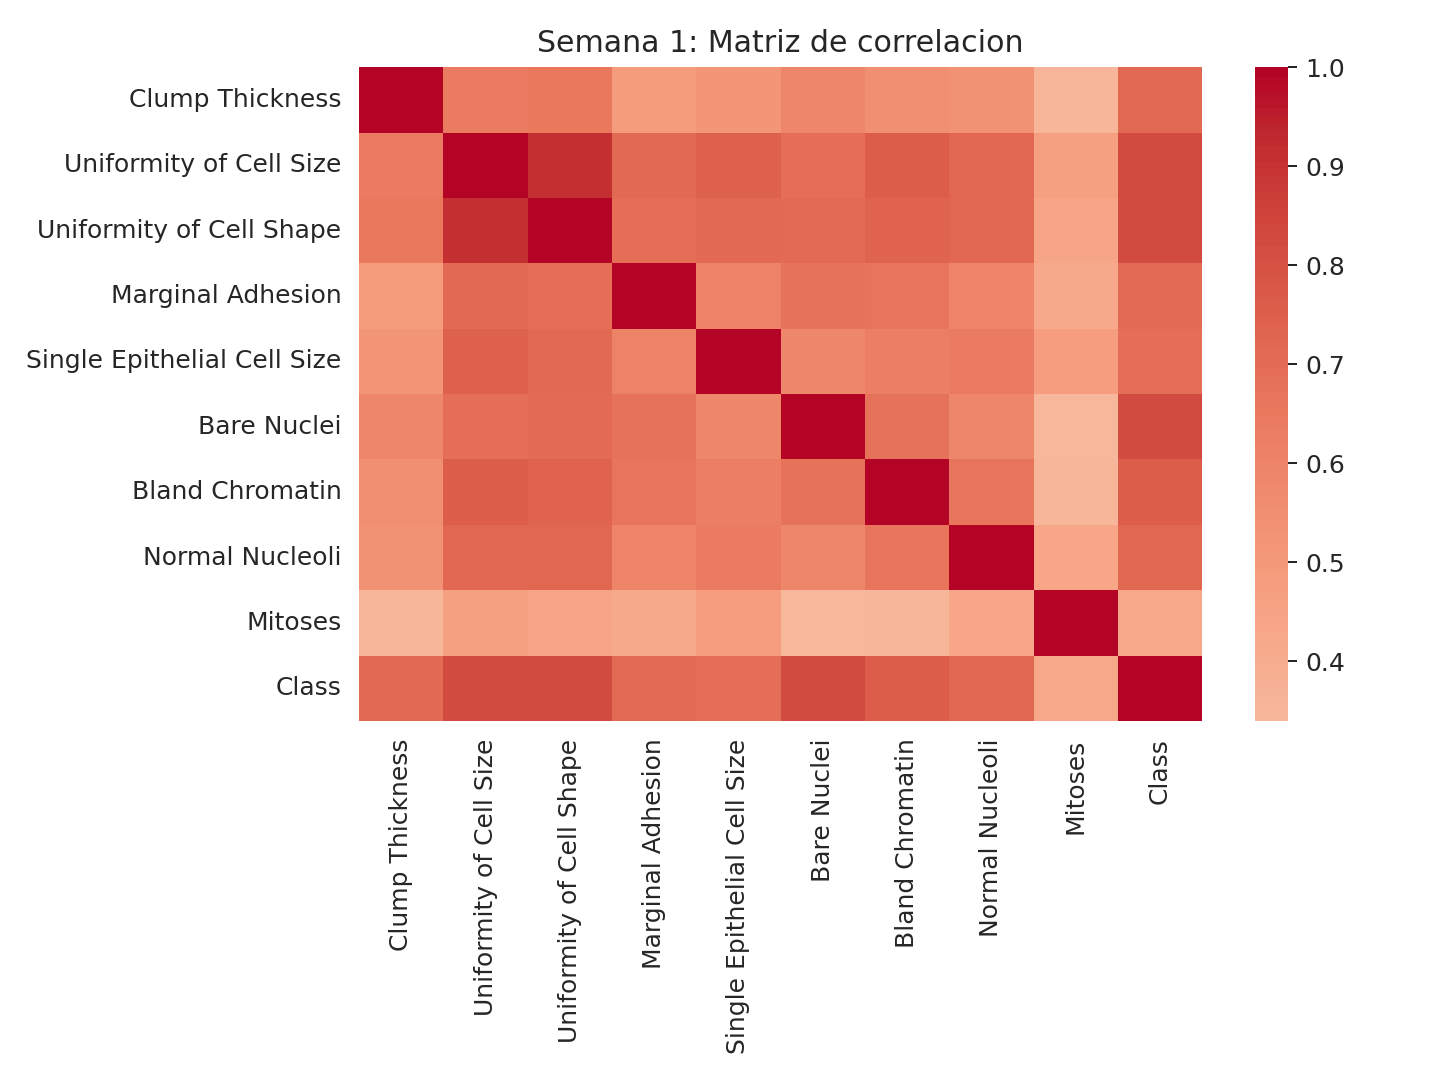
\includegraphics[width=0.88\textwidth]{figures/s1_correlacion_heatmap.png}
\caption{Matriz de correlación entre variables predictoras y variable objetivo. La esquina superior izquierda (variables de uniformidad) concentra la mayor colinealidad inter-variable.}
\end{figure}

\subsection{Análisis de outliers por clase}

Los outliers se calcularon aplicando el criterio IQR \textit{dentro de cada clase por separado}, evitando contaminar el umbral de normalidad de una clase con la distribución de la otra.

\begin{table}[H]
\centering
\caption{Conteo de outliers por variable y clase (IQR calculado dentro de cada clase)}
\renewcommand{\arraystretch}{1.1}
\begin{tabular}{lcccccc}
\toprule
\multirow{2}{*}{\textbf{Variable}} & \multicolumn{2}{c}{\textbf{Benigno (n=444)}} & \multicolumn{2}{c}{\textbf{Maligno (n=239)}} \\
\cmidrule(lr){2-3}\cmidrule(lr){4-5}
 & \textbf{N outliers} & \textbf{\%} & \textbf{N outliers} & \textbf{\%} \\
\midrule
Uniformity of Cell Shape & 100 & 22.5\% & 0 & 0.0\% \\
Single Epithelial Cell Size & 89 & 20.0\% & 0 & 0.0\% \\
Marginal Adhesion & 81 & 18.2\% & 0 & 0.0\% \\
Uniformity of Cell Size & 75 & 16.9\% & 0 & 0.0\% \\
Bare Nuclei & 57 & 12.8\% & 0 & 0.0\% \\
Normal Nucleoli & 53 & 11.9\% & 0 & 0.0\% \\
Mitoses & 13 & 2.9\% & 29 & 12.1\% \\
Bland Chromatin & 6 & 1.4\% & 0 & 0.0\% \\
\bottomrule
\end{tabular}
\end{table}

\textbf{Interpretación:} los outliers en la clase benigna corresponden a casos que, aun siendo benignos, presentan valores atípicamente altos en algunas variables citológicas. Son clínicamente plausibles (tumores benignos con rasgos atípicos). En la clase maligna, únicamente \texttt{Mitoses} genera outliers significativos (29, 12.1\%), consistente con la conocida relación entre alta actividad mitótica y tumores agresivos.

\textbf{Decisión metodológica:} no se eliminarán outliers de forma automática. Representan información clínica real que los modelos deben aprender a clasificar. Eliminarlos distorsionaría la distribución de los datos de entrenamiento.

\begin{figure}[H]
\centering
\includegraphics[width=\textwidth]{figures/s1_boxplots_por_clase.png}
\caption{Boxplots por diagnóstico de las 9 variables predictoras. Los puntos fuera de los bigotes representan outliers dentro de cada clase. La distribución de la clase maligna es visiblemente más dispersa en casi todas las variables.}
\end{figure}

\subsection{Separabilidad visual: variables discriminativas clave}

El análisis de las tres variables más correlacionadas con la clase (\texttt{Bare Nuclei}, \texttt{Uniformity of Cell Size}, \texttt{Uniformity of Cell Shape}) confirma fronteras de decisión visualmente claras:

\begin{figure}[H]
\centering
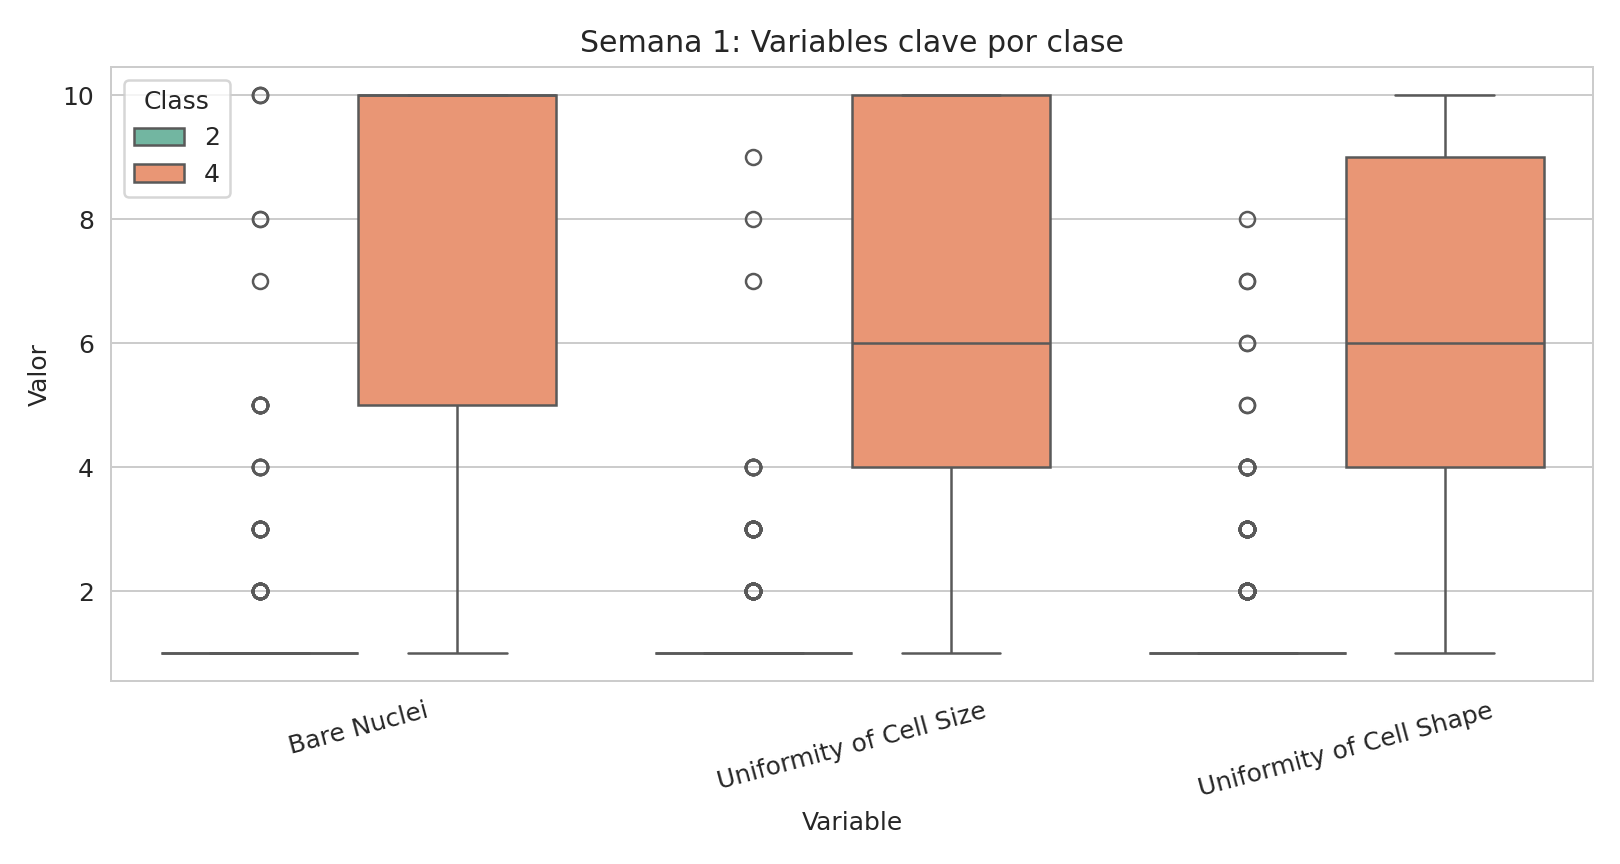
\includegraphics[width=0.9\textwidth]{figures/s1_boxplot_variables_clave.png}
\caption{Distribución de las tres variables más discriminativas por diagnóstico. Las medianas de la clase maligna son consistentemente entre 4 y 6 puntos más altas que las de la clase benigna.}
\end{figure}

\textbf{Decisión metodológica:} esta separabilidad respalda el uso de modelos con fronteras de decisión bien definidas (Regresión Logística y SVM). KNN se incluye como baseline no paramétrico para validar que la separabilidad no sea artefacto de un supuesto específico de distribución.

% ─────────────────────────────────────────────
\section{Plan de Acción Derivado del EDA}
% ─────────────────────────────────────────────

Cada hallazgo del EDA se traduce directamente en una decisión de diseño para Semana 2:

\begin{table}[H]
\centering
\caption{Mapa hallazgos EDA $\rightarrow$ decisiones de modelado}
\renewcommand{\arraystretch}{1.3}
\begin{tabularx}{\textwidth}{l X X}
\toprule
\textbf{Hallazgo EDA} & \textbf{Implicación técnica} & \textbf{Acción en Semana 2} \\
\midrule
\rowcolor{lightgray}
Separabilidad marcada por clase & Fronteras de decisión deben funcionar bien & Entrenar LR, KNN y SVM; esperar buen desempeño de todos \\
Colinealidad alta ($r=0.91$) & Riesgo de inestabilidad en modelos lineales & L2 en LR; Escenario B (top-3 variables) como prueba de robustez \\
\rowcolor{lightgray}
Desbalance 65/35 & Accuracy no es métrica confiable & \texttt{class\_weight=`balanced'}; priorizar Recall de maligna \\
Outliers clínicos en clase maligna & No son ruido; contienen información real & Conservar outliers; no aplicar limpieza agresiva \\
\rowcolor{lightgray}
Mitoses poco discriminativa & Puede añadir ruido & Evaluar en Escenario B si su exclusión mejora estabilidad \\
\bottomrule
\end{tabularx}
\end{table}

% ─────────────────────────────────────────────
\section{Hipótesis para el Modelado}
% ─────────────────────────────────────────────

Con base en el EDA, se establecen las siguientes hipótesis verificables en las semanas posteriores:

\begin{enumerate}[leftmargin=1.4cm, label=\textbf{H\arabic*.}]
\item \texttt{Bare Nuclei}, \texttt{Uniformity of Cell Size} y \texttt{Uniformity of Cell Shape} serán las features más importantes en cualquier modelo entrenado.
\item Modelos no lineales (SVM-RBF) capturarán mejor las relaciones del espacio de variables que modelos puramente lineales.
\item El Recall de la clase maligna debe ser la métrica de optimización principal, no la exactitud global.
\item La multicolinealidad entre variables de uniformidad puede desestabilizar modelos lineales sin regularización.
\item Los outliers clínicamente identificados (especialmente en \texttt{Mitoses} de la clase maligna) deben conservarse; eliminarlos perjudicaría el aprendizaje de casos agresivos.
\end{enumerate}

% ─────────────────────────────────────────────
\section{Síntesis de Semana 1}
% ─────────────────────────────────────────────

El EDA revela un dataset bien estructurado, sin valores nulos en variables predictoras y con separabilidad alta entre clases. Los hallazgos clave son tres: (1) las variables de uniformidad celular y los núcleos desnudos son los discriminadores más fuertes; (2) existe colinealidad considerable dentro del grupo de variables de uniformidad; y (3) el desbalance moderado exige estrategias de compensación y métricas centradas en la clase maligna.

El valor principal de esta semana no es descriptivo sino de diseño: cada hallazgo del EDA queda mapeado a una decisión concreta que condicionará el modelado de Semana 2 y la evaluación de Semana 3.

\vspace{1em}
\noindent\textbf{Repositorio del proyecto:}
\url{https://github.com/AngelEsquit/PRY2-MD.git}

\end{document}